\subsection{Performance Evaluation}
\label{sec:evaluation}

\begin{figure*}[tb]  % 星号*表示跨双栏
  \centering
    \renewcommand{\thesubfigure}{\roman{subfigure}} % 改为罗马数字
  % 第一行:横向两个子图
  \subfigure[\footnotesize Initial visit]{
    \begin{minipage}[b]{0.9\columnwidth}
      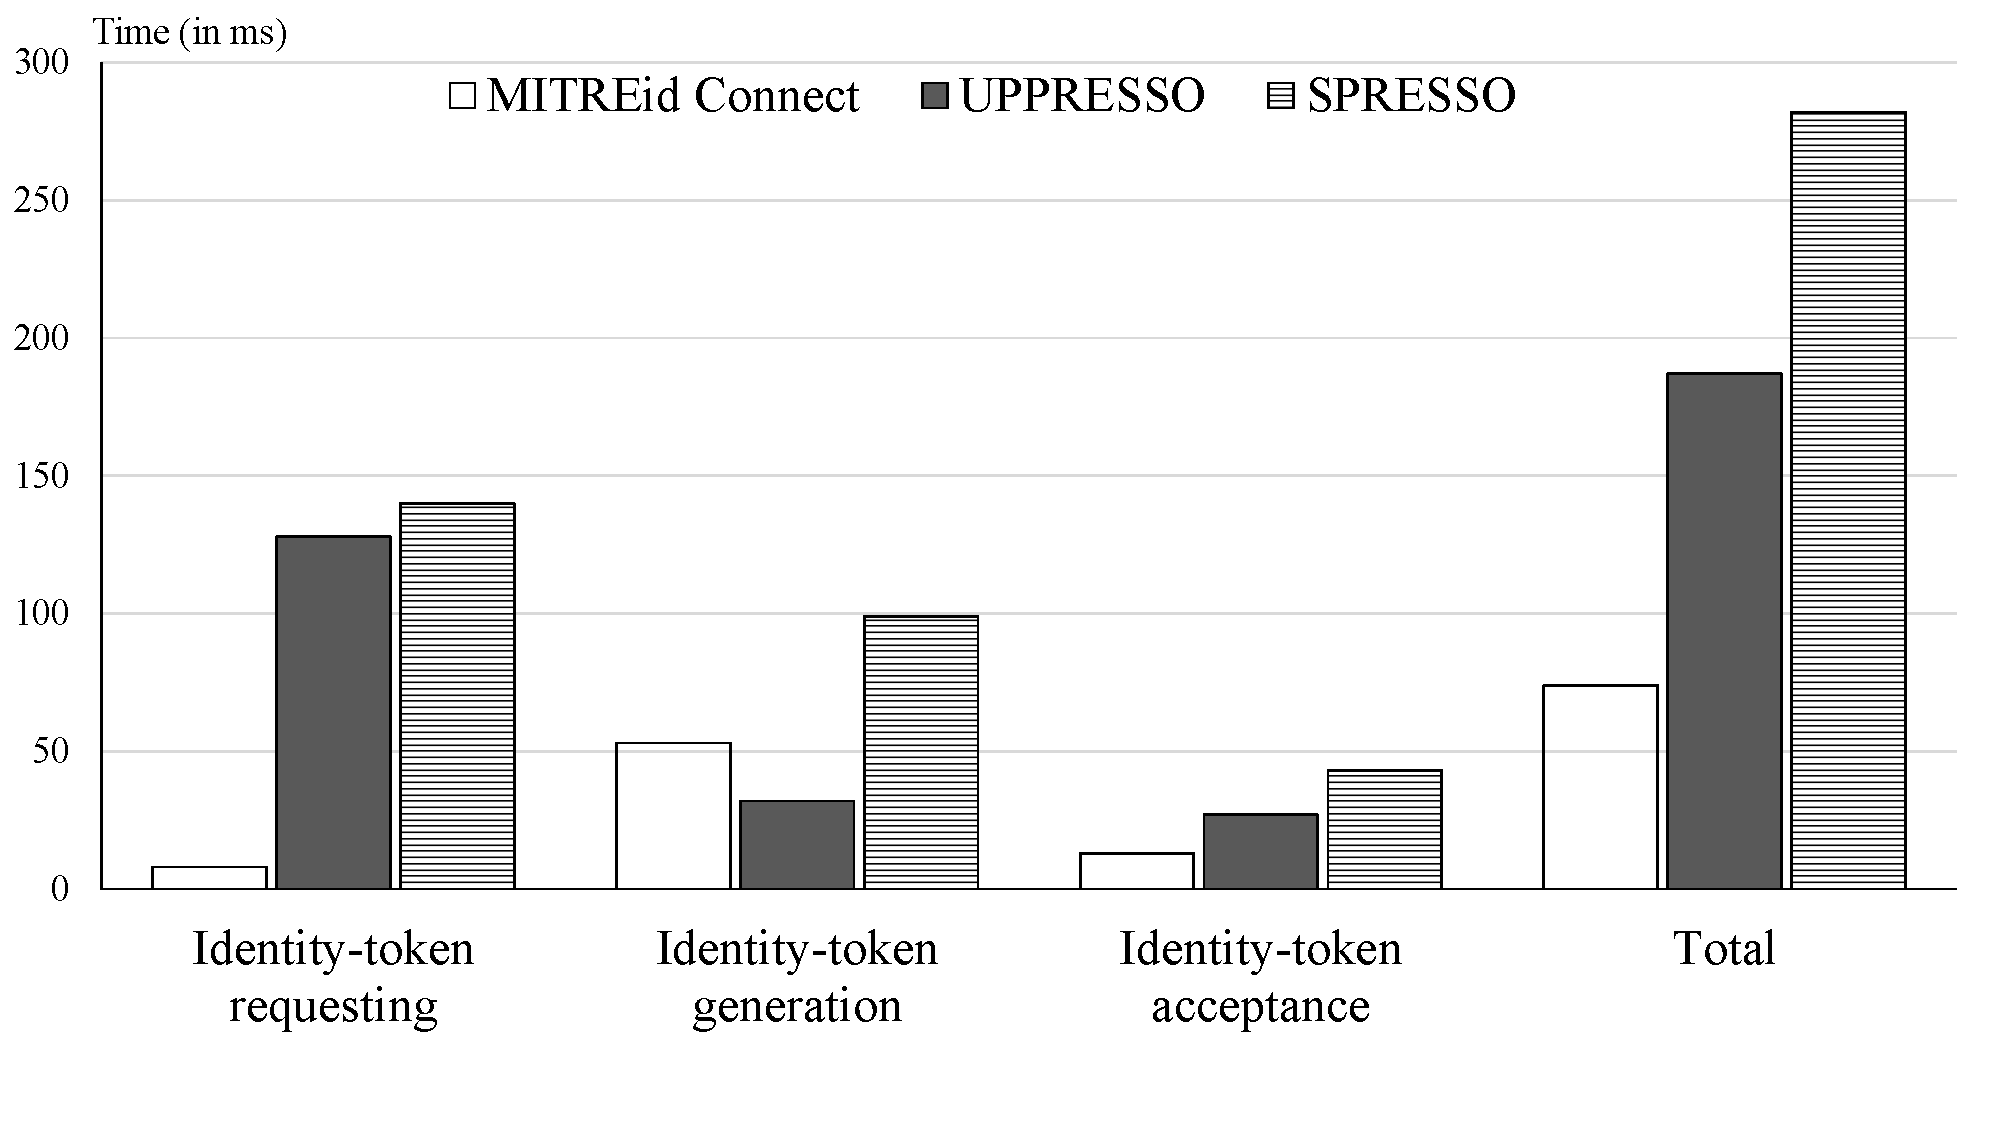
\includegraphics[width=\linewidth]{fig/evaluation-nocache-LAN.pdf}
    \end{minipage}
  }\hfill
  \subfigure[\footnotesize Subsequent visit]{
    \begin{minipage}[b]{0.9\columnwidth}
      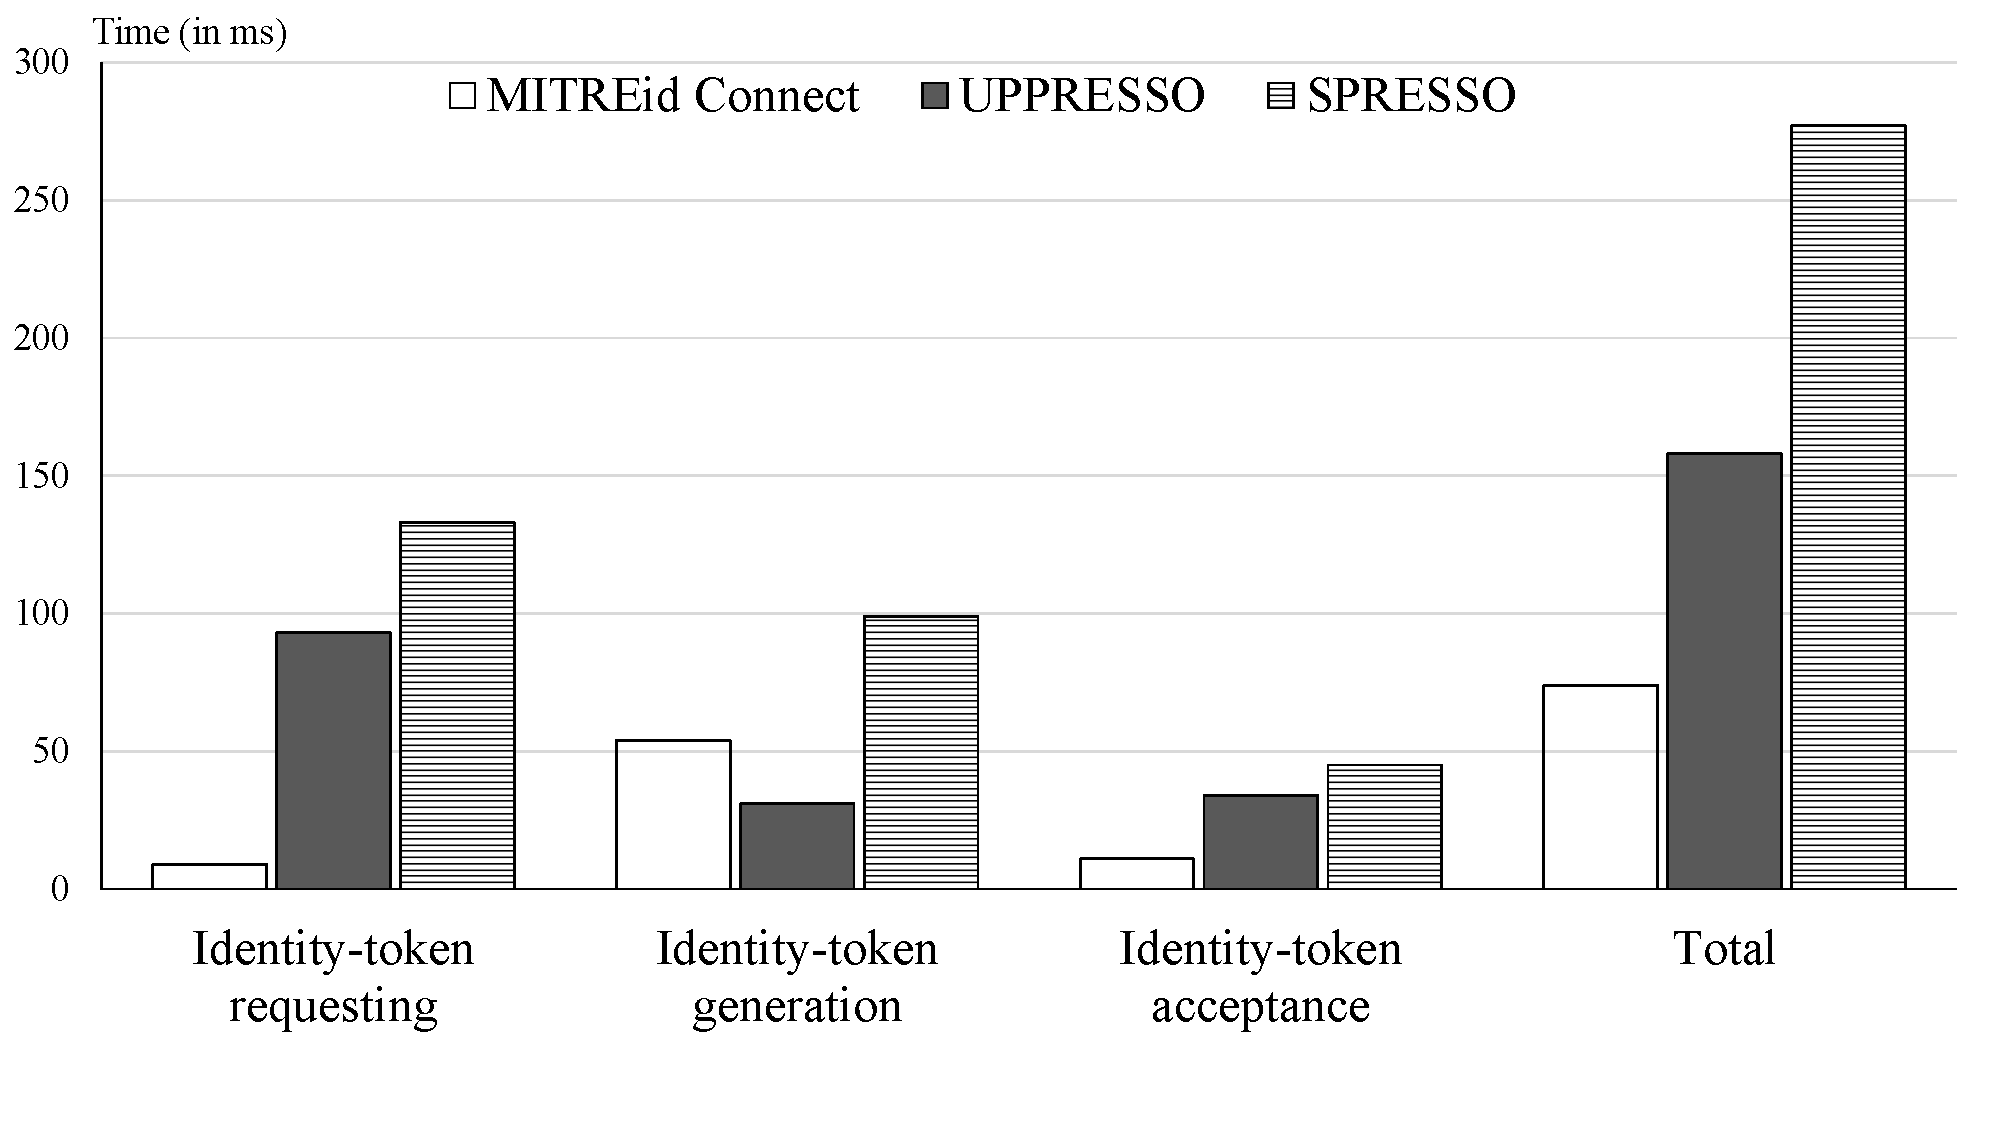
\includegraphics[width=\linewidth]{fig/evaluation-cache-LAN.pdf}
    \end{minipage}
  }
  \vspace*{-10pt}
  \par\medskip
  \centering{\footnotesize (a) Within a local virtual environment}

    \setcounter{subfigure}{0} % 重置subfigure计数器
  % 第二行:横向两个子图
  \subfigure[\footnotesize Initial visit]{
    \begin{minipage}[b]{0.9\columnwidth}
      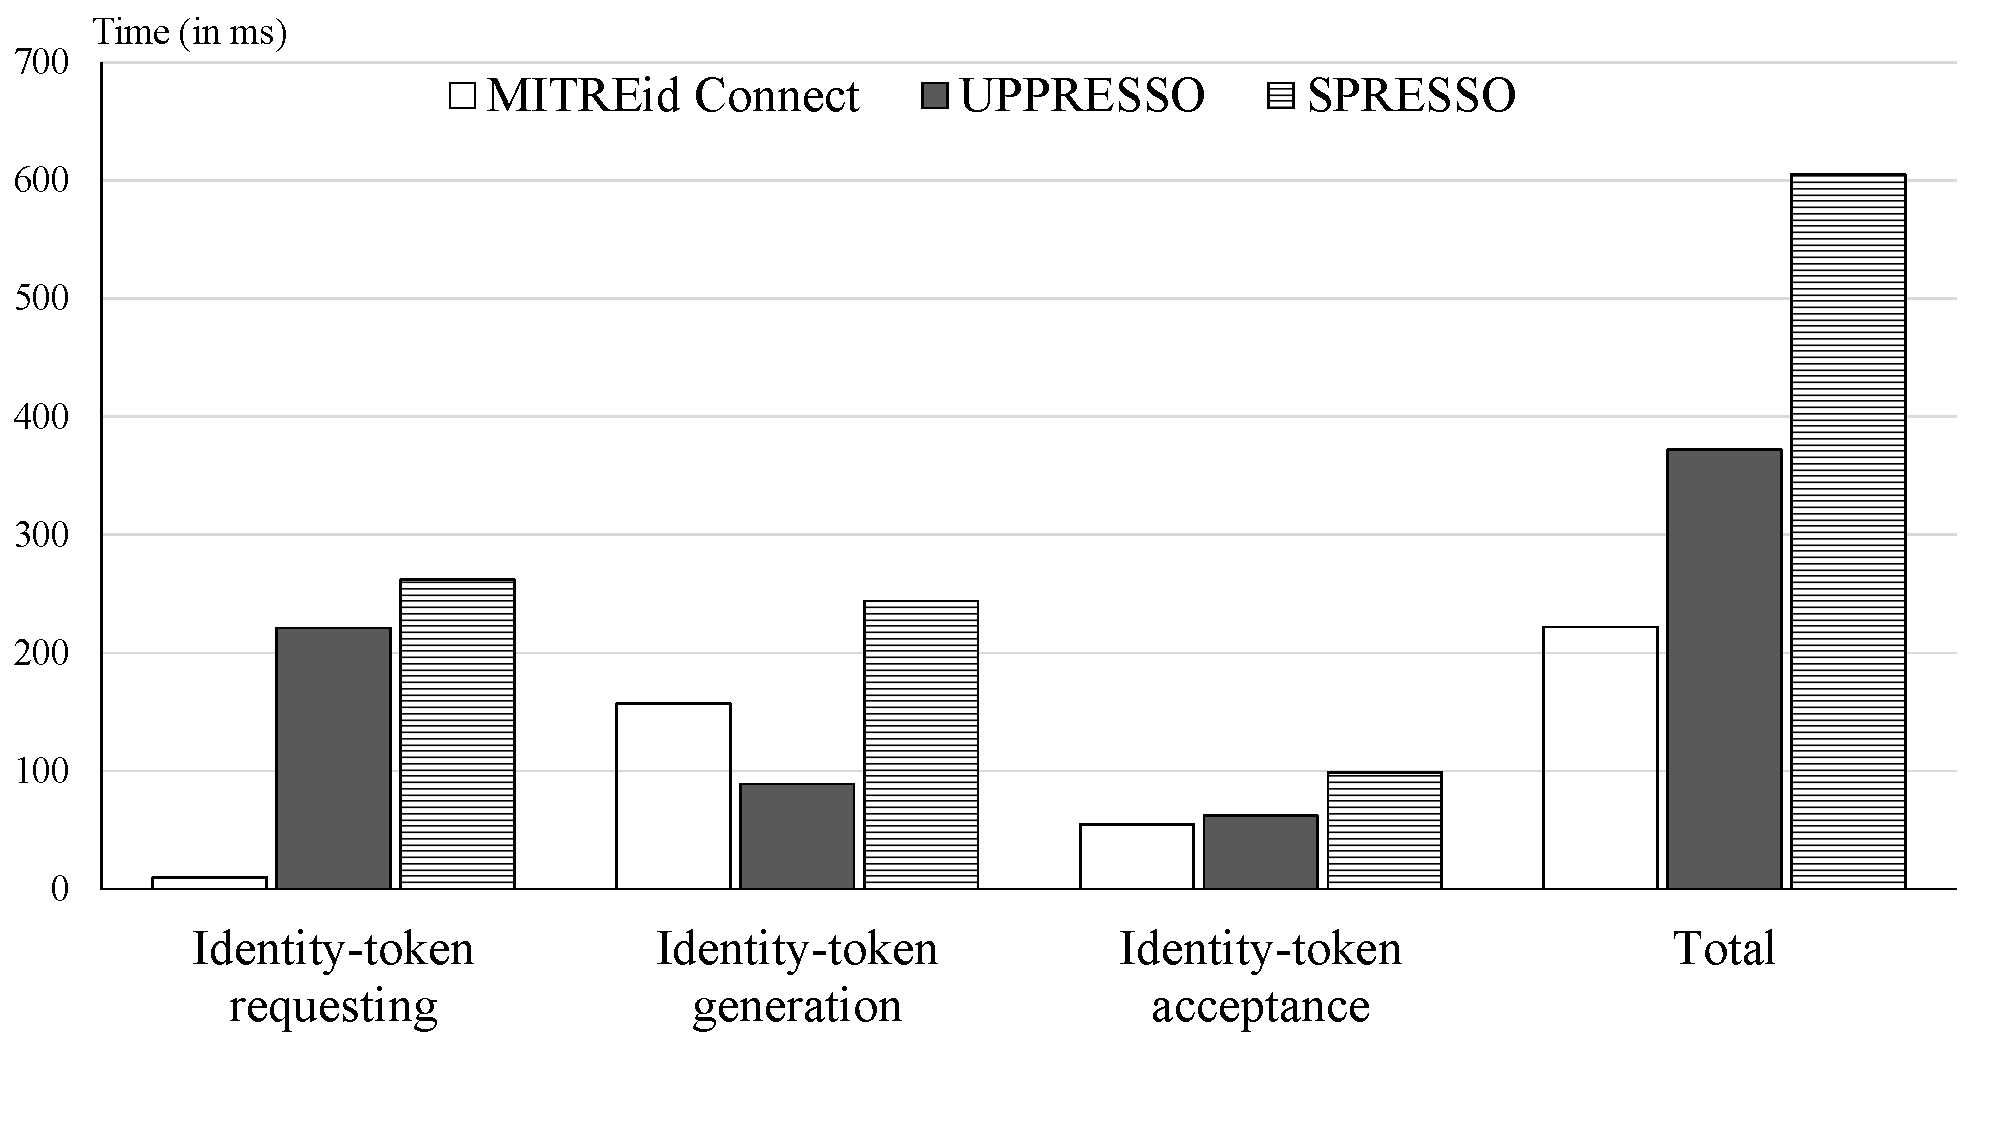
\includegraphics[width=\linewidth]{fig/evaluation-nocache-internet.pdf}
    \end{minipage}
  }\hfill
  \subfigure[\footnotesize Subsequent visit]{
    \begin{minipage}[b]{0.9\columnwidth}
      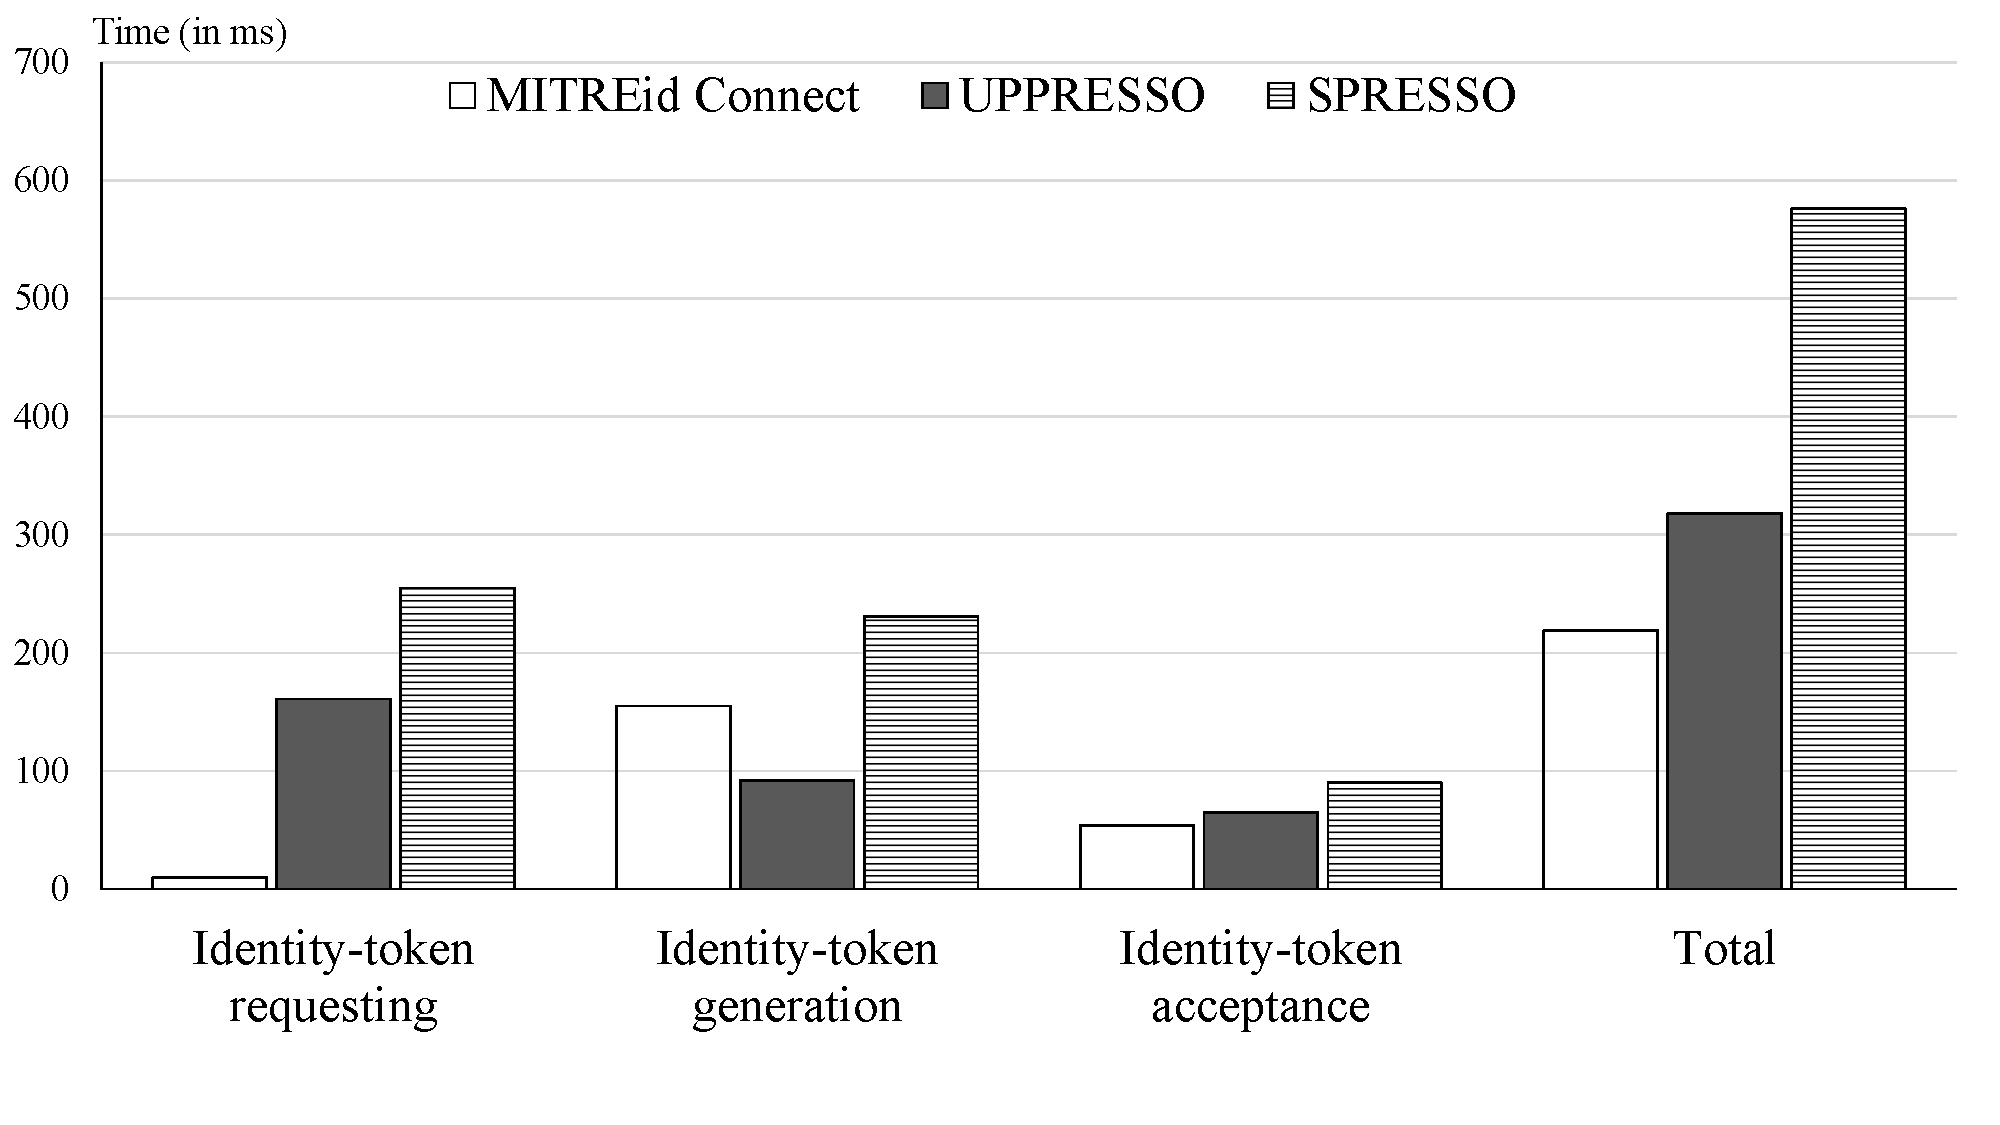
\includegraphics[width=\linewidth]{fig/evaluation-cache-internet.pdf}
    \end{minipage}
  }
  \vspace*{-10pt}
  \par\medskip
  \centering{\footnotesize (b) With a remotely-visiting browser}

  
  \vspace*{-5pt}
  \caption{The time costs of SSO login in MITREid Connect, UPPRESSO, and SPRESSO}
  \label{fig:evaluation}
\end{figure*} 

\noindent {\bf Experiment setting.}
%SPRESSO encrypts the RP's domain in identity tokens and keeps the AES symmetric key known only to the RP and the user.
We conducted experiments in two settings: (\emph{a}) on a PC with AMD Ryzen 7 57000X CPU and 32GB memory, a browser, the IdP, the visited RP, and the extra forwarder server of SPRESSO were deployed on separated virtual machines, each of which ran Windows Server 2025 with 2 vCPUs and 4GB RAM, and (\emph{b}) the browser running locally on the PC with AMD Ryzen 7 57000X CPU and 32GB memory, remotely accessed the servers (IdP and RP servers, and the forwarder server of SPRESSO) deployed on the Alibaba Cloud Elastic Compute Service, each of which ran Windows Server 2025 with 8 vCPUs and 32GB RAM. 
The first setting ran all functions on separated virtual machines but within the same physical PC,
    to minimize the impact of network delays.

%Of all solutions, the IdP and RP servers and the extra forwarder server of SPRESSO were all deployed on the Alibaba Cloud Elastic Compute Service, each of which ran Windows 10 with 8 vCPUs and 32GB RAM.

%We conducted experiments in two settings: (\emph{a}) a browser, Chrome 138.0.7204.158, ran on a virtual machine on the cloud platform with 8 vCPUs and 32 GB memory, and (\emph{b}) the browser running locally on a PC with Core i7-8700 CPU and 32 GB memory, remotely accessed the servers. All entities except the local browser, were deployed in the same virtual private cloud and connected to one vSwitch, which minimized the impact of network delays.
%In both settings, the IdP server never directly communicated with RPs.


\noindent {\bf Comparisons.} We split the login flow into three phases for detailed comparisons: (1)
{\em identity-token requesting} (Step 1 in Figure \ref{fig:process}), to construct an identity-token request and send it to the IdP server; (2) {\em identity-token generation} (Step 2), to generate an identity token at the IdP server, while the user authentication and the user-attribute consent are excluded; and (3) {\em identity-token acceptance} (Step 3), where the RP receives, verifies, and parses the identity token.


%\begin{figure}[tb]
 % \centering
%	\subfigure[In a virtual private cloud]{
%  		\begin{minipage}[b]{0.45\textwidth}
%			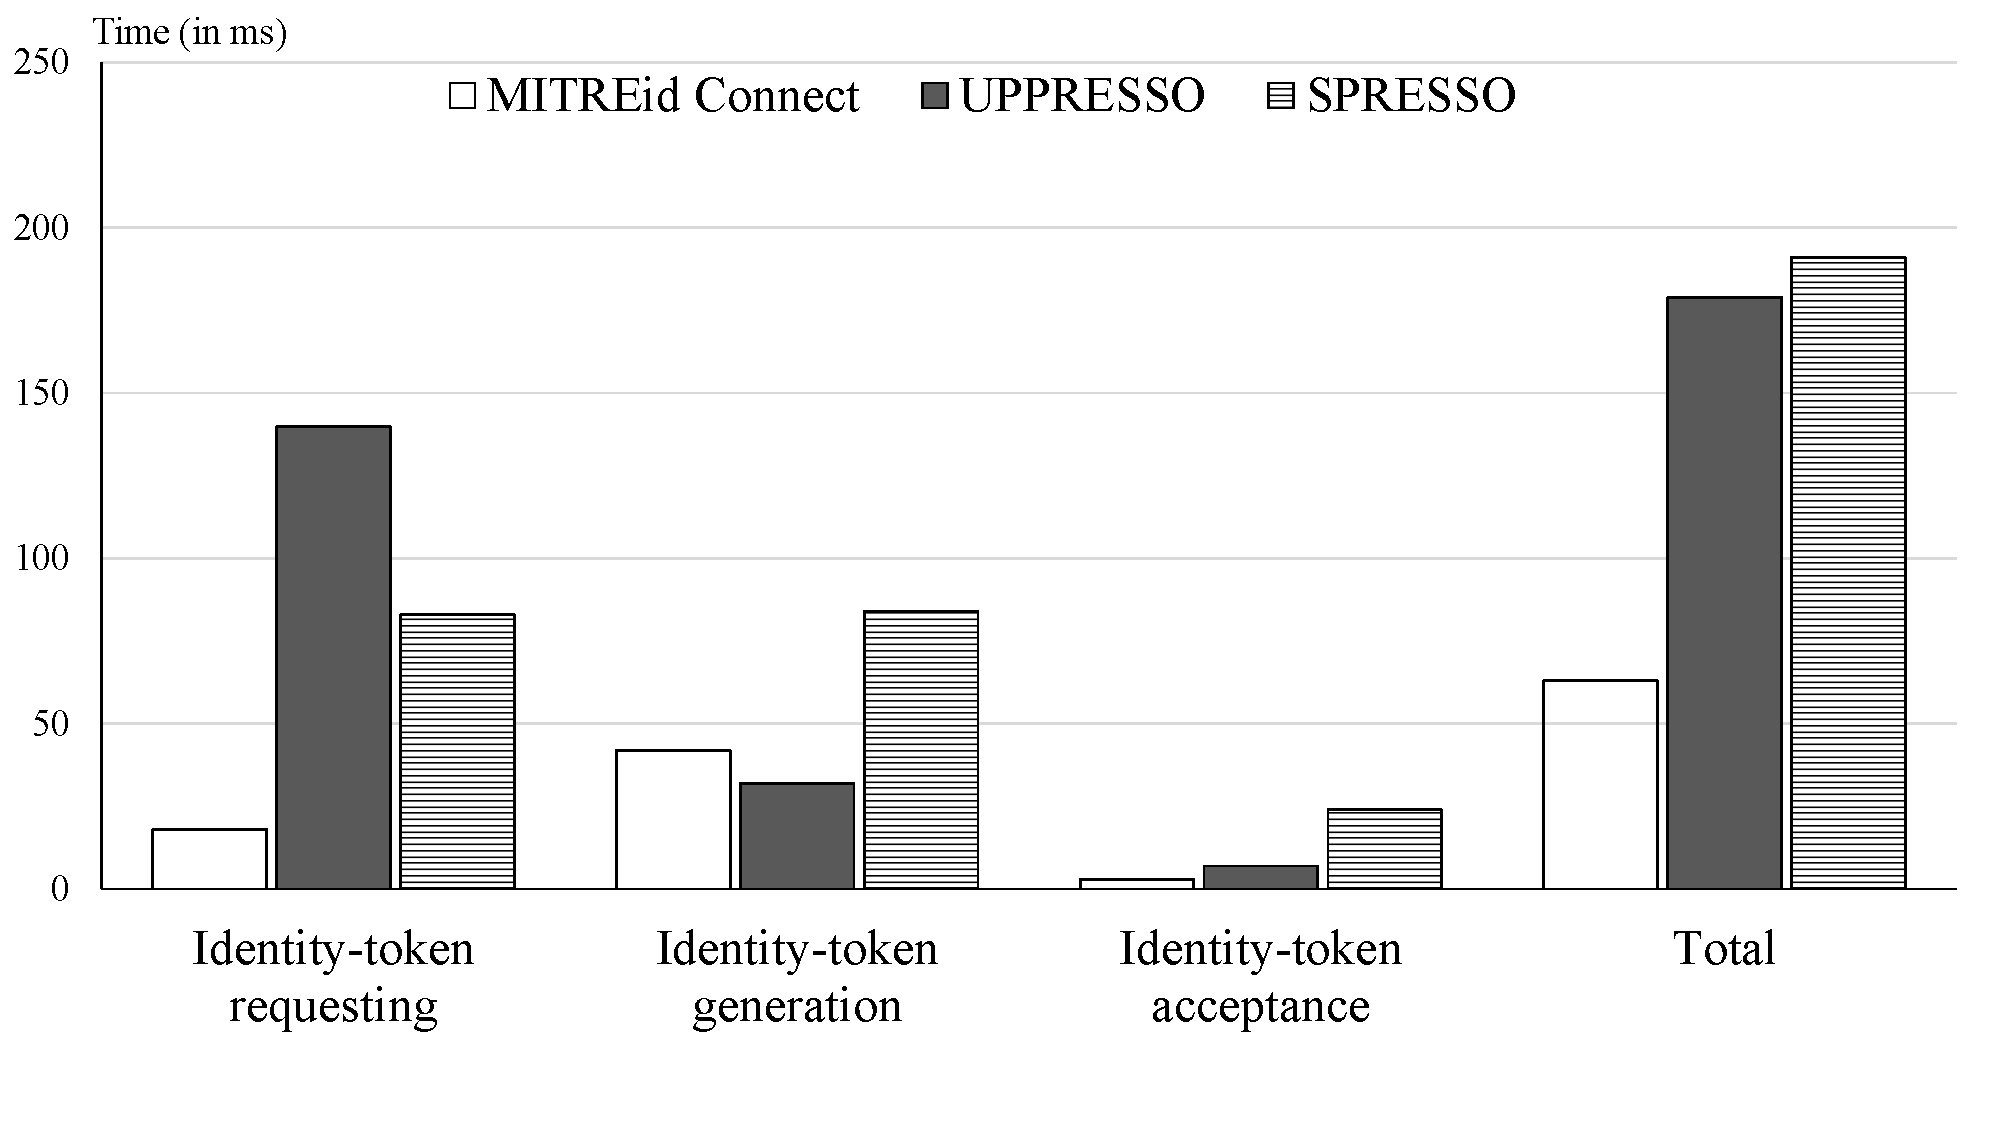
\includegraphics[width=0.97\linewidth]{fig/evaluation-lan.pdf}
%		\end{minipage}}
%	\subfigure[With a remotely-visiting browser]{
%  		\begin{minipage}[b]{0.45\textwidth}
%			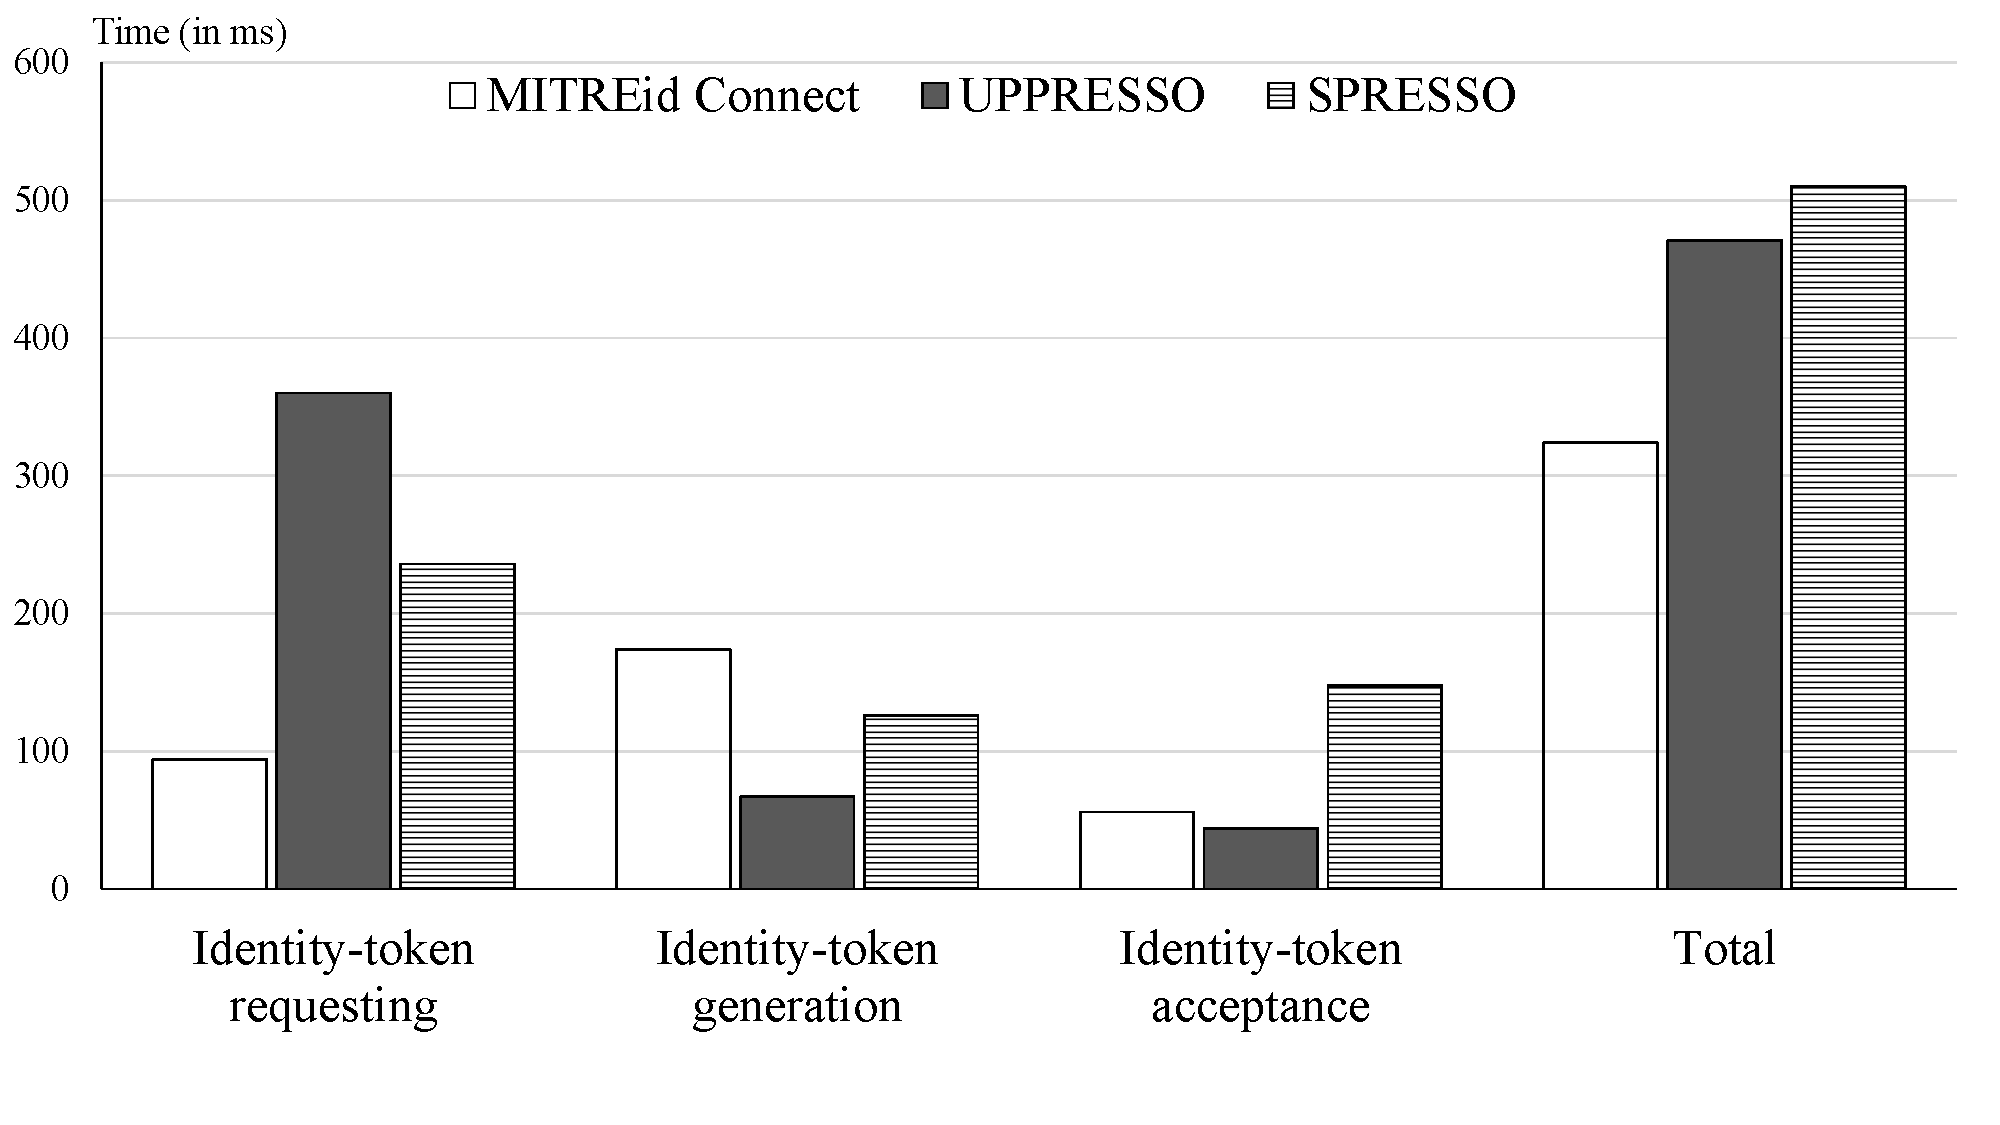
\includegraphics[width=0.97\linewidth]{fig/evaluation-internet.pdf}
%		\end{minipage}}
%  \caption{The time costs of SSO login in MITREid Connect, UPPRESSO, and SPRESSO}
%  \label{fig:evaluation}
%\end{figure}

The IdP and the RP of all solutions, as well as the forwarder server in SPRESSO,
     require user-side scripts, which introduces additional time for downloading. 
In the identity-token requesting phase of UPPRESSO a browser downloads the user-i script,
    as described in Section \ref{sec:web-design}.
As mentioned in Section \ref{subsec:OIDC},
 to process the token retrieved from the IdP, %which is carried with a URL following the fragment identifier \texttt{\#} instead of \texttt{?} due to security considerations \cite{de2014oauth},
    in MITREid Connect a user-r script is downloaded during the phase of token generation.
In addition to a script from the IdP in identity-token requesting,
SPRESSO needs another script from the forwarder server in the token acceptance phase \cite{SPRESSO}.
Fortunately, once a browser visits a web server, it caches the scripts locally, reducing the download time for subsequent visits.
This caching is enabled by the \verb+localStorage+ HTML object \cite{htmlStorageHtml} and HTTP  \texttt{Cache-Control} header.

Therefore, we measured the time cost for both initial and subsequent visits (1,000 trials) and compared the average SSO login times of three schemes.
As shown in Figure \ref{fig:evaluation},
MITREid Connect, UPPRESSO, and SPRESSO require (\emph{a}) 69 ms, 187 ms, and 282 ms for initial visits, and 74 ms, 158 ms and 277 ms for subsequent visits,
 or (\emph{b}) 222 ms, 372 ms, and 605 ms for initial visits, and 219 ms, 318 ms and 576 ms for subsequent visits.

Regarding identity-token requesting, %the user browser loads the RP's webpage and starts the login request.
the RP of MITREid Connect immediately constructs an identity-token request. %MITREid Connect only needs 10 ms but UPPRESSO requires 271 ms.
UPPRESSO incurs overheads in opening a new browser window and downloading the user-i script.
%
%\footnote{This pop-up overhead can be reduced %by silently conducting these operations when the user visits the RP website, or
%by browser extensions.
%We have implemented such a browser extension while keeping the IdP and RPs unmodified, and the supplementary experiments showed a reduction of (\emph{a}) about 90 ms in the virtual private cloud setting and (\emph{b}) 260 ms when accessed remotely.}
%
In SPRESSO the user also needs to open a new browser window, and obtain information about the IdP % 's public key %(SPRESSO allows a user to assign any IdPs before login without initial registrations)
and encrypt the visited RP's domain using an ephemeral key, resulting in extra overheads.

UPPRESSO requires the least time for generating identity tokens for it receives the token from the IdP without additional processing.
In this phase MITREid Connect and SPRESSO require extra time as the browser downloads a script from the RP and the forwarder, respectively. % to process the token retrieved from the IdP, which is carried with a URL following the fragment identifier \texttt{#} instead of \texttt{?} due to security considerations \cite{de2014oauth}.
After receiving an identity token from the IdP, in SPRESSO the user decrypts the RP's domain by scripts and sends it to the RP's redirection endpoint.
Moreover, SPRESSO takes slightly more time to generate an identity token, as it implements the IdP using node.js and uses a JavaScript cryptographic library that is a little less efficient than the Java library used in the others.

Finally, in the identity-token acceptance phase, 
three solutions take similar amounts of time for the RP to receive a token and accept it.
% In contrast, SPRESSO takes the longest time due to its complex processing at the user agent.


By comparing the average time costs of initial visits and subsequent visits,
    we find that the performances of all schemes are improved
        and the improvement is the most significant in UPPRESSO for the size of its scripts is the largest. 